%%%%%%%%%%%%%%%%%%%%%%%%%%%%
%%%%%%%%%%%%%%%%%%%%%%%%%%%%
\chapter{\LaTeX\ Help}
\label{ch:Help}
%%%%%%%%%%%%%%%%%%%%%%%%%%%%


In this chapter, I will show you how to use some of the commands and packages in the template for PhD theses. The following topics will be explained:

\begin{itemize}
	\item What is in the file \texttt{localcommands} and how can I use the commands? (Sec.~\ref{ch:Commands})
	
	\item How can I work with the package \texttt{lsp-gb4eMyP} for examples? (Sec.~\ref{ch:Examples})
	
	\item How can I add information (e.g.\ sources) to examples \texttt{jambox}? (Sec.~\ref{ch:TextPositioning})
		
	\item How can I insert figures and tables with floating environments? (Sec.~\ref{ch:FigTab})
	
	\item Which entry types can I use for bibliographical information? (Sec.~\ref{ch:BibEntries} \& \ref{ch:CitationCommands})
		
	\item Abbreviations and indices (Sec.~\ref{ch:Indices})

	\item How can I add personal notes to my text? (Sec.~\ref{ch:Notes})

	\item How can I use the new environment for chapter notes? (Sec.~\ref{ch:Chapternotes})	

	\item Further helpful \LaTeX\ literature (Sec.~\ref{ch:HelpLiterature})
\end{itemize}


Take into account that this is not an introduction into \LaTeX . For a short \LaTeX\  introduction in German, see \citet{Freitag&MyP15a}.


%%%%%%%%%%%%%%%%%%%%%%%%%%%%
%%%%%%%%%%%%%%%%%%%%%%%%%%%%
\section{Own commands}
\label{ch:Commands}
%%%%%%%%%%%%%%%%%%%%%%%%%%%%

In the file \texttt{texfiles/localcommands} you can define your own commands. I have pre-defined some commands such that you can see how that works.

\begin{itemize}
	\item \verb|\zB| renders the German abbreviation \zB (for `for example'), with a protected blank between ``z.'' and ``B.''.
	
	\item \verb|\gqq{argument}|  renders the German double quotation marks, as in \gqq{argument}.
	
	\item \verb|\gq{argument}|  renders the German single quotation marks, as in \gq{argument}.
	
	\item The commands \verb|\red{argument}| and \verb|\blue{argument}| render text in blue or red, e.g.\ \red{argument}, \blue{argument}.
	
	\item The commands \verb|\clrr{argument}| and \verb|\clry{argument}| render text marked with red  or yellow, e.g.\ \clrr{argument}, \clry{argument}.
\end{itemize}


%%%%%%%%%%%%%%%%%%%%%%%%%%%%
%%%%%%%%%%%%%%%%%%%%%%%%%%%%
\section{Examples}
\label{ch:Examples}
%%%%%%%%%%%%%%%%%%%%%%%%%%%%


In this document, the package \texttt{langsci-gb4e} is loaded%
	%
	\footnote{All packages are loaded in the file \texttt{texfiles/localpackages}.} %
	%
for creating example environments.
It is a slightly modified version of \texttt{gb4e}, see the \texttt{gb4e} manual \citep{Kolb&Co10a} or \citet{Freitag&MyP15a}) for further explanations.
\texttt{langsci-gb4e} can be used with the same \LaTeX \ syntax as \texttt{gb4e}:


\begin{lstlisting}
\begin{exe}
\ex This is an example.
\ex This is the second example.
  \begin{xlist}
    \ex embedded examples with different numbering
    \ex These examples are numbered with letters.
    \ex another example numbered with letters
  \end{xlist}
\end{exe}
\end{lstlisting}


\noindent \texttt{langsci-gb4e} also provides a somewhat simpler syntax:

\begin{lstlisting}
\ea This is an example.
\ex This is the second example.
  \ea embedded examples with different numbering
  \ex These examples are numbered with letters.
  \ex another example numbered with letters
  \z   
\z
\end{lstlisting}


The result in both cases is the same:

\ea This is an example.

\ex This is the second example.

	\ea embedded examples with different numbering
	
	\ex These examples are numbered with letters.
	
	\ex another example numbered with letters
	\z   
\z


%%%%%%%%%%%%%%%%%%%%%%%%%%%%
%%%%%%%%%%%%%%%%%%%%%%%%%%%%
\section{Figures and Tables}
\label{ch:FigTab}
%%%%%%%%%%%%%%%%%%%%%%%%%%%%


There is a floating environment for figures. It is floating but you can (try to) fix%
	%
	\footnote{If there is not enough place where you want to position the graphic, \LaTeX\ will choose a different place, e.g.\ at the top of the next page.} %
	%
the figure on a position with the option \texttt{[h]}. The environment is helpful to center figures using the command \verb|\centering| and to add captions that are listed in the List of Figures.%
	%
	\footnote{For more on figures, tables, and captions, see \citet{Freitag&MyP15a}.} %
	%

By using the command \verb|\includegraphics| from the package \texttt{graphicx} you can include graphics. All you have to do is indicate the graphic's file path (see the Figure~\ref{fig:Frege}).


\begin{lstlisting}
\begin{figure}[h]
  \centering
  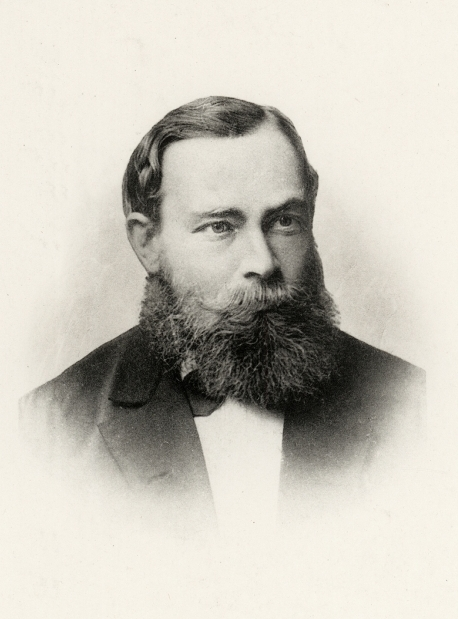
\includegraphics[scale=.45]{graphics/Young-Frege}
  \caption{Young Frege}
  \label{fig:Frege}
\end{figure}
\end{lstlisting}


\begin{figure}[h]
	\centering
	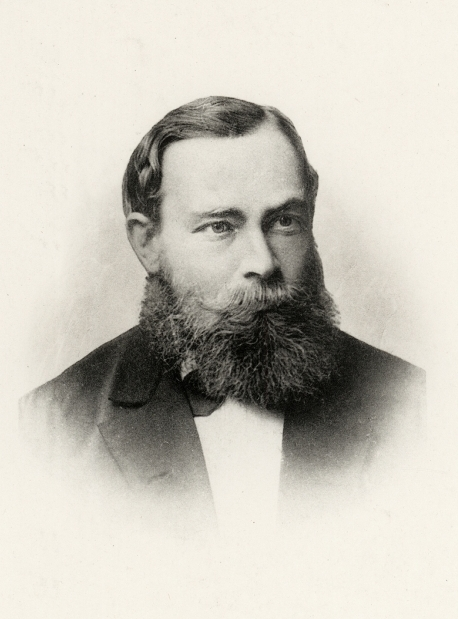
\includegraphics[scale=.45]{graphics/Young-Frege}
	\caption{Young Frege}
	\label{fig:Frege}
\end{figure}


\noindent It works in the same way for tables.


\begin{lstlisting}
\begin{table}[h]
  \centering
  \begin{tabular}{l|l}
    Figure & Table \\
    \hline
    test & test \\
  \end{tabular}
  \caption{Test table}
\end{table}
\end{lstlisting}


\begin{table}[h]
	\centering
	\begin{tabular}{l|l}
		Figure & Table \\
		\hline
		test & test \\
	\end{tabular}
	\caption{Test table}
\end{table}


%%%%%%%%%%%%%%%%%%%%%%%%%%%%
%%%%%%%%%%%%%%%%%%%%%%%%%%%%
\section{Examples for different bibliographical entries}
\label{ch:BibEntries}
%%%%%%%%%%%%%%%%%%%%%%%%%%%%


In order to see which information you need in your Bib\TeX\ file for different entry types%
	%
	\footnote{See also \url{https://en.wikipedia.org/wiki/BibTeX} or \citet{Freitag&MyP15a}.} %
	%
(e.g.\ article, book, manuscript, etc.), check the file \texttt{texfiles/literature}.%
	%
	\footnote{The file \texttt{texfiles/literature} is the Bib\TeX\ file for this document. You can introduce your entries there.} %
	%
If you want to see the output for every specific entry type (e.g.\ \texttt{phdthesis} vs.\ \texttt{book}), take a look at the bibliography of this PDF.


\begin{itemize*}
	\item PhD Thesis: \citet{Abney87a}
	
	\item Article in an edited book: \citet{Ackema15a}
	
	\item Book: \citet{Adger04a}
	
	\item Edited book: \citet{Nolda&Co14a}
	
	\item Article in a journal: \citet{Barwise&Co81a}
	
	\item Article in an online journal or database:
	\citet{Kolb&Co10a}
	
	\item Unpublished work / manuscript: \citet{MyP17c}
	
	\item Published work without author, using a key, i.e.\ an abbreviation for the citation (this can be used e.g.\ for corpora or dictionaries): \citep{DR17a}
	
	\item Published entry in an encyclopedia (online): \citet{MyP18b}
\end{itemize*}


%%%%%%%%%%%%%%%%%%%%%%%%%%%%
%%%%%%%%%%%%%%%%%%%%%%%%%%%%
\section{Examples for different citation commands with \texttt{natbib}}
\label{ch:CitationCommands}
%%%%%%%%%%%%%%%%%%%%%%%%%%%%

The package \texttt{natbib} (loaded in \texttt{texfiles/localpackages}) provides different commands for citations. You can find the IDs for every bibliography entry in the file \texttt{texfiles/literature}, but they are also being suggested as soon as you type in one of the \verb|\cite| commands.


\vspace{.5cm}


\begin{footnotesize}

\begin{tabular}{p{7cm}|p{5.6cm}}
	\textbf{input} & \textbf{output} \\
	\midrule
	\verb|\citep{Heim&Kratzer00a}| & {\citep{Heim&Kratzer00a}} \\
	
	\verb|\citep[cf.][4--5]{Heim&Kratzer00a}| & {\citep[cf.][4--5]{Heim&Kratzer00a}} \\
	
	 \verb|\citet{Heim&Kratzer00a}| & {\citet{Heim&Kratzer00a}} \\

	\verb|\citep[cf.][]{Heim&Kratzer00a}| & {\citep[cf.][]{Heim&Kratzer00a}} \\

	\verb|\citep[56--76]{Heim&Kratzer00a}| & {\citep[56--76]{Heim&Kratzer00a}} \\

	\verb|\citealp[56]{Heim&Kratzer00a}| & {\citealp[56]{Heim&Kratzer00a} }\\

	\verb|\citealt[43ff]{Heim&Kratzer00a}| &{\citealt[43--45]{Heim&Kratzer00a}} \\

	\verb|\citep{Heim&Kratzer00a,Abney87a}|  & {\citep{Heim&Kratzer00a,Abney87a}} \\
\end{tabular}

\end{footnotesize}


%%%%%%%%%%%%%%%%%%%%%%%%%%%%
%%%%%%%%%%%%%%%%%%%%%%%%%%%%
\section{Abbreviations and indices}
\label{ch:Indices}
\index{index|(} 
%%%%%%%%%%%%%%%%%%%%%%%%%%%%


For further information about indices, take a look at the documentation of the package \texttt{imakeidx}%
	%
	\footnote{\url{https://ctan.org/pkg/imakeidx}.} %
	%
and the Wikipedia page for indices.%
%
\footnote{\url{https://en.wikibooks.org/wiki/LaTeX/Indexing}} %
%

For abbreviations, the package \texttt{acronym}%
%
\footnote{\url{https://ctan.org/pkg/acronym}.} %
%
is very useful and easy to implement. First the abbreviations are defined (see Section Abbreviations) and then used with the command \verb|\ac{acronym}|.  The pre-defined acronyms in the Section Abbreviations are: 

\begin{itemize}
\item \ac{acc}, 
\item \ac{CP}, 
\item \ac{dat},  
\item \ac{IPA} 
\end{itemize}


%%%%%%%%%%%%%%%%%%%%%%%%%%%%
%%%%%%%%%%%%%%%%%%%%%%%%%%%%
\section{Notes}
\label{ch:Notes}
%%%%%%%%%%%%%%%%%%%%%%%%%%%%


If you want to write preliminary margin notes, \todo{This note is orange.} you can use the command \verb|\todo|.%
	%
	\footnote{Take a look at the documentation of the package \url{https://ctan.org/pkg/todonotes}. You can customise your own to-do notes.} %
	%


%%%%%%%%%%%%%%%%%%%%%%%%%%%%
%%%%%%%%%%%%%%%%%%%%%%%%%%%%
\section{Helpful literature}
\label{ch:HelpLiterature}
%%%%%%%%%%%%%%%%%%%%%%%%%%%%


When writing your term paper / thesis, you can take a look at the following literature for further help (German explanations are for texts in German):


\begin{itemize*}
	\item \citet{DR17a}: Für Fragen zur Rechtschreibung 
	
	\item \citet{MyP17c} oder \citet{Rothstein11a}: Für Fragen bzgl.\ der Fertigstellung von Hausarbeiten
	
	\item \citet{Haspelmath14a}: General style rules for linguistic papers
	
	\item \citet{LeipzigGloss15a}: Glossing rules
	
	\item \citet{Freitag&MyP15a}: Für Fragen bzgl.\ \LaTeX\
	
	\item \citet{Kolb&Co10a}: For questions regarding the syntax of \texttt{gb4e}
	
\end{itemize*}